\documentclass{article}
\usepackage{graphicx}
\begin{document}
\title{Tutorial I$^2$C device}
\maketitle
\section{Device pinout}
The device has 4 pins connected as described in picture~(\ref{l-pinout}).
\begin{figure}[h]
  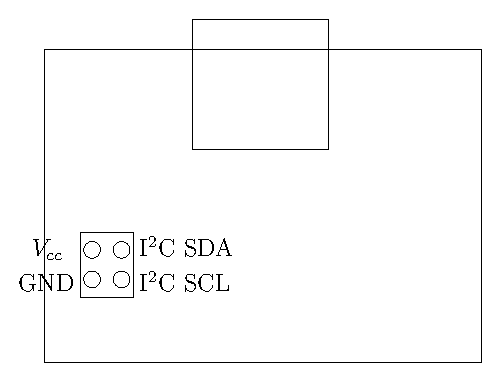
\includegraphics[width=3cm]{pinout}
  \caption{Device pinout. $V_{cc}$ pin is supply voltage. GND pin should be connected to the ground. Two other pins are for I$^2$C communication}\label{l-pinout}
\end{figure}
\section{Device communication protocol}
\subsection{I$^2$C protocol description}
The device communicates via two-wire I$^2$C interface as a slave device. The device use 7-bit addressing mode. The data rate in the standard mode is limited to 10kbps. The default (factory) device slave address is 0x33 (8-bit address 0x66 for writing 0x67 for reading). 

The device include pull-up resistors between $V_{cc}$ pin and I$^2$C lines.

All bus transactions begin with the master device issuing the start sequence followed by the slave address byte. The address byte contains the slave address: the upper 7-bits is the 7-bit slave address, followed by one bit which is set to 1 if the operation is read and to 0 if the operation is write. At the 9-th clock pulse the receiving slave device will issue ACK (by pulling the SDA line low) or NACK. Following these bus events, the master will send out bytes for a write operation, or the slave will clock out data with the read operation.All bus transactions are terminated with the master issuing a stop sequence. 

\subsection{SMBus protocol description}
The device use subset of SMBus protocol to transfer the values of its registers to the master device.
\subsubsection{Key to symbols}
\begin{tabular}{lll}
  S    & (1 bit) & Start bit\\
  P    & (1 bit) & Stop bit\\
  Rd/Wr & (1 bit) & Read/Write bit. Rd equals 1, Wr equals 0.\\
  A, NA & (1 bit) & Accept and reverse accept bit. \\
  Addr  & (7 bits)& I2C 7 bit address.\\
  Comm  & (8 bits)& Register(command) \\
  Data  & (8 bits)& A plain data byte. \\
  $[$...$]$  &         & Data send by slave as opposed to data send by master
\end{tabular}

\subsubsection{Reading a register}
The following sequence reads a single byte from the device register:

S Addr Wr [A] Comm [A] S Addr Rd [A] [Data] NA P

\subsection{Writing a register}
The following sequence writes a single byte to the device register:

S Addr Wr [A] Comm [A] Data [A] P

\subsubsection{Reading a block of registers}

\subsubsection{Writing a block of registers}


\section{Registers description}

\paragraph{Resistor readout register: address 0x03}
Contains value corresponding to the current position of resistor sensor. Value is in range 0..255. Read-only, write operations will be ignored.
\paragraph{Semi-random value register: address 0x05}
The value of this register is continuously updated. Suitable to getting semi-random numbers in the range 0..127.
Read-only, write operations will be ignored.
\paragraph{Identification register: address 0x06}
The value read from this register is always constant -- decimal 50.
Read-only, write operations will be ignored.
\paragraph{LED control register: address 0x07}
Writing non-zero value to this register switches LED on. Writing zero to this register swithches LED off. Reading from this register will give the status of the LED.
Read-write.


\end{document}
